\documentclass[a4paper,]{article}
\usepackage[left=2.5cm,top=2.5cm,right=2.5cm,bottom=3cm]{geometry} 
\usepackage[utf8]{inputenc}
\usepackage{graphicx} % Required for inserting images
\usepackage[table,xcdraw]{xcolor}
\usepackage{lipsum} % for dummy text
\usepackage{mathdots} % para el comando \iddots
\usepackage{mathrsfs} % para formato de letra
\usepackage{ marvosym }


\title{\textbf{HW0: Introduction to Financial Engineering}}
\author{Miguel Angel Aguilo Gonzalez, 1699413 \\ Judit de Paz Ramírez, 1570590 \\ Laia Mòdol Rodríguez, 1565282 \\ Elena Rubio Zabala, 1699049 \\ Guillem Tutusaus Alcaraz, 1533701 } 
\date{Octubre 2023}

\begin{document}

\maketitle
\newpage

\section*{Ejercicio 1}
El análisis de los rendimientos diarios netos de acciones individuales y de índices bursátiles desempeña un papel fundamental en la toma de decisiones financieras y en la comprensión de los movimientos del mercado. En este informe examinaremos los rendimientos diarios netos de las acciones de Google (GOOG) y del índice compuesto S$\&$P (SP) durante el período comprendido entre el 3 de enero de 2011 y el 31 de diciembre de 2014.
\\

El análisis de los rendimientos diarios netos es esencial para los inversionistas y analistas, éste nos proporciona información valiosa sobre la volatilidad, el rendimiento y la correlación de activos financieros. Al observar estas tendencias, intentaremos comparar y esperar que los datos se comporten como una distribución conocida.\\

El objetivo principal de este informe será reproducir una prueba de normalidad sobre los rendimientos netos diarios y registrar los rendimientos del precio de cierre de las acciones de Google y el índice compuesto S$\&$P.  Para ello estudiaremos algunas estadísticas básicas que nos ofrecen información predictiva útil, éstas se encuentran recogidas en la siguiente tabla:\\

% TABLA PARÀMETROS NET RETURNS
\begin{table}[h]
\centering
\begin{tabular}{ccccccc}
\hline
\rowcolor[HTML]{C0C0C0} 
\multicolumn{1}{|c|}{\cellcolor[HTML]{C0C0C0}Return} & \multicolumn{1}{c|}{\cellcolor[HTML]{C0C0C0}Media} & \multicolumn{1}{c|}{\cellcolor[HTML]{C0C0C0}Desv. típica} & \multicolumn{1}{c|}{\cellcolor[HTML]{C0C0C0}Asimetría} & \multicolumn{1}{c|}{\cellcolor[HTML]{C0C0C0}Exceso cortosis} & \multicolumn{1}{c|}{\cellcolor[HTML]{C0C0C0}Mínimo} & \multicolumn{1}{c|}{\cellcolor[HTML]{C0C0C0}Máximo} \\ \hline
\multicolumn{1}{|c|}{\cellcolor[HTML]{EFEFEF}GOOG}   & \multicolumn{1}{c|}{0.00067596}                  & \multicolumn{1}{c|}{0.01518733}                                   & \multicolumn{1}{c|}{0.8204034}                         & \multicolumn{1}{c|}{14.2879}                                    & \multicolumn{1}{c|}{-0.08377501}                    & \multicolumn{1}{c|}{0.1379628}                      \\ \hline
\multicolumn{1}{|c|}{\cellcolor[HTML]{EFEFEF}SP}     & \multicolumn{1}{c|}{0.00043237}                  & \multicolumn{1}{c|}{0.01918323}                                   & \multicolumn{1}{c|}{0.06868225}                        & \multicolumn{1}{c|}{2.547833}                                   & \multicolumn{1}{c|}{-0.08246155}                    & \multicolumn{1}{c|}{0.09507754}                     \\ \hline
\multicolumn{1}{l}{}                                 & \multicolumn{1}{l}{}                               & \multicolumn{1}{l}{}                                              & \multicolumn{1}{l}{}                                   & \multicolumn{1}{l}{}                                            & \multicolumn{1}{l}{}                                & \multicolumn{1}{l}{}                               
\end{tabular}
\end{table}

Continuaremos el estudio mediante un análisis grafico utilizando los datos de la rentabilidad neta de las acciones de Google. Para ello nos será muy útil la función de densidad empírica, ésta es otra herramienta predictiva usada para observar el comportamiento de una muestra. \\

Observando la siguiente gráfica podemos pensar que los datos siguen una distribución normal con valor de media igual a cero, sin embargo, este argumento no es valido para aceptar la hipótesis.

\begin{figure}[h!]
    \centering
    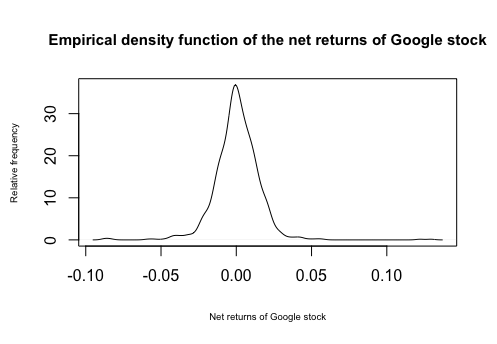
\includegraphics[scale=0.65]{Rplot1.png}
\end{figure}

Así pues, aplicaremos un contraste de bondad de ajuste para ver si nuestros datos empíricos pueden seguir una distribución normal. Usando la prueba de Shapiro-Wilk planteamos como hipótesis nula que nuestra muestra proviene de una población normalmente distribuida y observamos que obtenemos en el p-valor. Si el p-valor es menor a 0.05 entonces la hipótesis nula es rechazada (se concluye que los datos no vienen de una distribución normal). Si el p-valor es mayor a 0.05, se concluye que no se puede rechazar dicha hipótesis.\\

El p-valor que obtenemos al realizar la prueba es menor que $2.2e^{-16}$, este hecho es suficiente para rechazar nuestra hipótesis nula y poder afirmar que el rendimiento neto de las acciones de Google no sigue una distribución normal.  \\

Cuando se trabaja con precios o índices de mercado habitualmente es utilizada la transformación o rendimiento logarítmico. Su uso proviene de las propiedades de continuidad que tiene. Hagamos de nuevo la tabla con las estadísticas básicas usando el rendimiento logarítmico para mejorar los datos conseguidos.



% TABLA PARAMETROS LOG RETURNS
\begin{table}[h!]
\centering
\begin{tabular}{ccccccc}
\hline
\rowcolor[HTML]{C0C0C0} 
\multicolumn{1}{|c|}{\cellcolor[HTML]{C0C0C0}Return} & \multicolumn{1}{c|}{\cellcolor[HTML]{C0C0C0}Media} & \multicolumn{1}{c|}{\cellcolor[HTML]{C0C0C0}Desv. típica} & \multicolumn{1}{c|}{\cellcolor[HTML]{C0C0C0}Asimetría} & \multicolumn{1}{c|}{\cellcolor[HTML]{C0C0C0}Exceso cortosis} & \multicolumn{1}{c|}{\cellcolor[HTML]{C0C0C0}Mínimo} & \multicolumn{1}{c|}{\cellcolor[HTML]{C0C0C0}Máximo} \\ \hline
\multicolumn{1}{|c|}{\cellcolor[HTML]{EFEFEF}GOOG}   & \multicolumn{1}{c|}{0.00056142}                  & \multicolumn{1}{c|}{0.01510793}                                   & \multicolumn{1}{c|}{0.4859664}                         & \multicolumn{1}{c|}{12.44483}                                    & \multicolumn{1}{c|}{-0.08749332}                    & \multicolumn{1}{c|}{0.1292397}                      \\ \hline
\multicolumn{1}{|c|}{\cellcolor[HTML]{EFEFEF}SP}     & \multicolumn{1}{c|}{0.00024860}                  & \multicolumn{1}{c|}{0.01917923}                                   & \multicolumn{1}{c|}{-0.06076117}                        & \multicolumn{1}{c|}{2.475171}                                   & \multicolumn{1}{c|}{-0.08606079}                    & \multicolumn{1}{c|}{0.09082517}                     \\ \hline
\multicolumn{1}{l}{}                                 & \multicolumn{1}{l}{}                               & \multicolumn{1}{l}{}                                              & \multicolumn{1}{l}{}                                   & \multicolumn{1}{l}{}                                            & \multicolumn{1}{l}{}                                & \multicolumn{1}{l}{}                               
\end{tabular}
\end{table}

Ahora, para estudiar la distribución de los datos, consideraremos que nuestra nueva muestra sigue una distribución normal. Realizamos la prueba T de Student de los datos de Google para probar la hipótesis nula (la media es 0) y, de la misma manera que con la prueba Shapiro-Wilk, decidiremos si refutar o quedarnos con la hipótesis. \\

El p-valor que obtenemos en este caso es de $0.2393>0.005$, por lo tanto, no podemos rechazar la hipótesis nula. Para poder garantizar que esto es cierto, calcularemos la función de densidad empírica de ambos datos y realizaremos de nuevo la prueba Shapiro-Wilk. \\


Si graficamos la función de densidad empírica tenemos: 
\begin{figure}[h!]
    \centering
    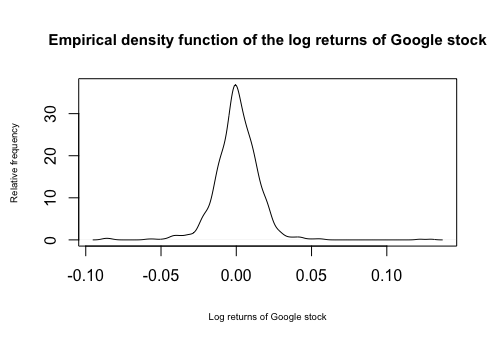
\includegraphics[scale=0.55]{Rplot2.png}
    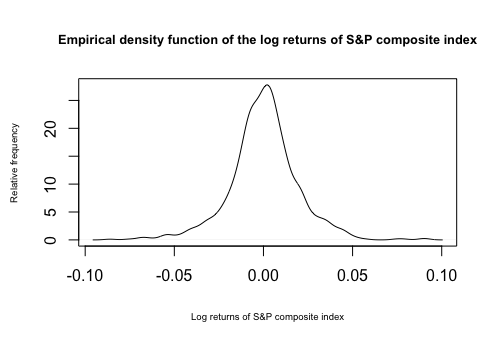
\includegraphics[scale=0.55]{Rplot3.png}
\end{figure}

Al realizar la prueba Shapiro-Wilk conseguimos un p- valor $2.2e^{-16}<0.05$, y de $4.963e^{-14}$ por lo que en los dos casos refutamos la hipótesis nula y, por lo tanto, ninguna sigue la distribución normal. \\

Finalmente, buscaremos el intervalo de confianza del $95\%$ de los datos de las acciones de Google. Para ello, pese a no seguir una distribución normal, usaremos el T-test, ya que es lo que da una mejor aproximación. 
El intervalo que hemos conseguido es el siguiente: $$(-0.0003742273, 0.0014970606)$$

\newpage
\section*{Ejercicio 2}
Supongamos que nos encontramos en la siguiente situación, encontramos nuestra casa perfecta pero nos faltan 240.000 euros, por lo que, necesitamos un préstamo del banco que pagaremos durante 30 años. Por el préstamo, pagas un interés de $1.99\%$ al año. Queremos calcular cuanto tendremos que pagar al mes, para ello utilizaremos la siguiente fórmula:

$$D\frac{R}{12}+\frac{D\frac{R}{12}}{(1+\frac{R}{12})^{12T}-1}$$

Donde D es el dinero, R es el interés y T el tiempo (en años). En nuestro caso D=240000, R=1.99 y T=30. \\

Sustituyendo estos valores en la fórmula anterior, conseguimos lo que tendremos que pagar al mes, que es 885,887 euros.\\

Además, con R podemos construir la tabla que resuma lo que tendremos que pagar cada año.\\

\begin{table}[h!]
\centering
\begin{tabular}{|
>{\columncolor[HTML]{EFEFEF}}c |c|c|c|}
\hline
\cellcolor[HTML]{C0C0C0}Año & \cellcolor[HTML]{C0C0C0}Deuda al inicio del período & \cellcolor[HTML]{C0C0C0}Intereses acumulados & \cellcolor[HTML]{C0C0C0}Capital reembolsado \\ \hline
1                           & 240.000,00                                          & 4.722,30                                     & 5.908,34                                    \\ \hline
2                           & 234.091,66                                          & 4.603,65                                     & 6.026,99                                    \\ \hline
3                           & 228.064,67                                          & 4.482,61                                     & 6.148,03                                    \\ \hline
4                           & 221.916,63                                          & 4.359,15                                     & 6.271,50                                    \\ \hline
5                           & 215.645,13                                          & 4.233,20                                     & 6.397,45                                    \\ \hline
6                           & 209.247,69                                          & 4.104,72                                     & 6.525,92                                    \\ \hline
7                           & 202.721,76                                          & 3.973,66                                     & 6.656,98                                    \\ \hline
8                           & 196.064,78                                          & 3.839,98                                     & 6.790,67                                    \\ \hline
9                           & 189.274,11                                          & 3.703,60                                     & 6.927,04                                    \\ \hline
10                          & 182.347,07                                          & 3.564,49                                     & 7.066,16                                    \\ \hline
11                          & 175.280,91                                          & 3.422,58                                     & 7.208,06                                    \\ \hline
12                          & 168.072,85                                          & 3.277,83                                     & 7.352,82                                    \\ \hline
13                          & 160.720,03                                          & 3.130,16                                     & 7.500,48                                    \\ \hline
14                          & 153.219,55                                          & 2.979,54                                     & 7.651,11                                    \\ \hline
15                          & 145.568,44                                          & 2.825,88                                     & 7.804,76                                    \\ \hline
16                          & 137.763,68                                          & 2.669,14                                     & 7.961,50                                    \\ \hline
17                          & 129.802,18                                          & 2.509,26                                     & 8.121,39                                    \\ \hline
18                          & 121.680,79                                          & 2.346,16                                     & 8.284,49                                    \\ \hline
19                          & 113.396,30                                          & 2.179,78                                     & 8.450,86                                    \\ \hline
20                          & 104.945,44                                          & 2.010,07                                     & 8.620,58                                    \\ \hline
21                          & 96.324,87                                           & 1.836,95                                     & 8.793,70                                    \\ \hline
22                          & 87.531,17                                           & 1.660,35                                     & 8.970,30                                    \\ \hline
23                          & 78.560,87                                           & 1.480,20                                     & 9.150,44                                    \\ \hline
24                          & 69.410,43                                           & 1.296,44                                     & 9.334,21                                    \\ \hline
25                          & 60.076,22                                           & 1.108,98                                     & 9.521,66                                    \\ \hline
26                          & 50.554,56                                           & 917,76                                       & 9.712,88                                    \\ \hline
27                          & 40.841,68                                           & 722,71                                       & 9.907,94                                    \\ \hline
28                          & 30.933,74                                           & 523,73                                       & 10.106,92                                   \\ \hline
29                          & 20.826,82                                           & 320,76                                       & 10.309,89                                   \\ \hline
30                          & 10.516,94                                           & 113,71                                       & 10.516,94                                   \\ \hline
\end{tabular}
\end{table}

Despues de los 30 años, habremos pagado al banco 318.919,30 euros y como solo necesitabamos 240.000 euros pagamos de más 78.919,34 euros al banco. \\

%LA D: EXPLICACION Y OTRA TABLA
Supongamos ahora que el banco nos ofrece pagar un interés inicial del 1.99\%, distribuido en un \textit{market index} (1\%) y una \textit{spread} (0.99\%). El \textit{spread} es fijo a lo largo de la totalidad del crédito, mientras que el \textit{market index} va incrementando un 0.1\% cada año que pasa. De este modo, al final del crédito el interés será del 4.89\%. Calculando el dinero que hemos pagado al banco al final de estos 30 años obtenemos la suma total de 363.655,30 euros. Con este nuevo crédito pagamos de más 123.655,30 euros.



\end{document}



